\documentclass[a4paper,openright,12pt]{book}
\usepackage{graphicx}
\usepackage[sort&compress]{natbib}
\usepackage[spanish]{babel}
\usepackage{epsfig}
\usepackage{rotating}
\usepackage{amsmath}
\usepackage{slashbox}
\usepackage{setspace}
\usepackage{amsfonts}
\usepackage{dcolumn}
\usepackage{multirow}
\usepackage{url}
\usepackage{natbib}
\usepackage{amssymb}
\usepackage{times}
\usepackage{fontspec}
\usepackage{booktabs}
\usepackage{geometry}
\usepackage{cite}
\usepackage{caption}
% \usepackage[utf8]{inputenc}

\setcounter{secnumdepth}{3}
\setmainfont{Times New Roman}
\geometry{left=3cm,right=3cm,top=2.5cm,bottom=2.5cm}

\RequirePackage{ifpdf} % ¿latex o pdflatex?
% Configuración de las imágenes

\usepackage{graphicx}		% Inclusión de imágenes
\DeclareGraphicsExtensions{.eps}

\graphicspath{ {../imgs/} } % Ruta respecto al fichero tex principal dónde se buscan imágenes

\onehalfspace
\begin{document}

\begin{titlepage}

\begin{center}
\vspace*{-1in}
\begin{figure}[htb]
\begin{center}

\includegraphics[height=2cm]{logo_uz}
\hfill
\includegraphics[height=2cm]{logo_fecem}
\end{center}
\end{figure}
\vspace*{0.15in}
FACULTAD DE CIENCIAS ECONÓMICAS Y EMPRESARIALES \\
\vspace*{0.15in}
DEPARTAMENTO DE ESTRUCTURA ECONÓMICA\\
\vspace*{0.6in}
\begin{large}
TRABAJO\\
\end{large}
\vspace*{0.2in}
\begin{Large}
\textbf{COMERCIO INTERNACIONAL} \\
\end{Large}
\vspace*{0.3in}
\begin{large}
Análisis De La Economía De Chipre \\ 
\end{large}
\vspace*{0.3in}
%\rule{80mm}{0.1mm}\\
%\vspace*{0.1in}
\begin{large}
Autor: \\
Maximiliano Greco \\
\end{large}
\end{center}

\end{titlepage}

\newpage




% -------------- EMPIEZA LA READACCIÓN-----------------------------------------

\chapter{Presentación Del País}
\label{cap1}


\section{Situación Geográfica}


\begin{figure}[htb]
    \centering
    \caption{Situación geográfica de Chipre.}
    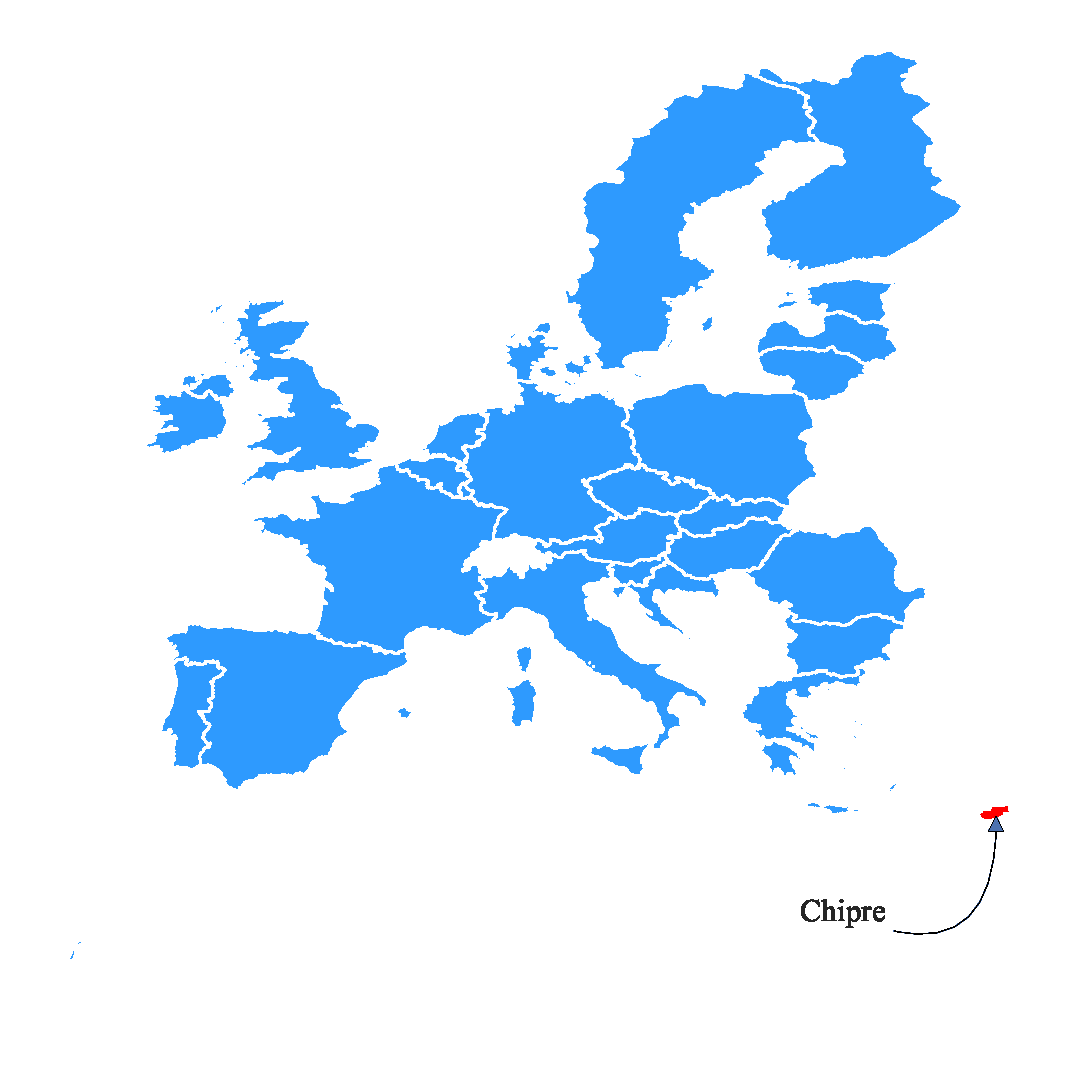
\includegraphics[width=9cm]{mapa}
    \caption*{\textit{Fuente}: Elaboración propia a partir de Shapefile de Eurostat}
    \label{fig1}
\end{figure}

\section{Historia}

Chipre tiene una riqueza histórica que comienza en la prehistoria, desde pozos de agua mas antiguos del mundo[cita], hasta poblados del neolítico[cita]. Chipre ha albergado a diversas cultaras, cómo la Griega y la fenicia (Antigua región orginalmente que en la actualidad iba desde Israel hasta Siria), pasando por Egipcios, persas, el imperio romano, Bizantino (actual Turquía), Árabe, Rep. de Venecia, Turco-Otomana, británica y griega otra vez. En 1974 se produce un golpe de estado por el gobierno Turco, invadiendo el tercio norte de Chipre, y dando origen a la Rep. Turca del Norte de Chipre (RTNC) que es un estado que sólo reconoce Turquía. En 2004 Chipre entra en la Unión Europea.

Chipre se divide en seis distritos:

\begin{enumerate}

    \item Nicosia: Se encuentra en la RTNC
    \item Famagusta: Se encuentra en la RTNC
    \item Limassol
    \item Pafos
    \item Lárnaca
    \item Kyrenia: Se encuentra en la RTNC
\end{enumerate}

 Además, en el sur existen dos territorios que son bases militares bajo el mando de Reino Unido.

\begin{enumerate}
    \item Acrotiri
    \item Dhekelia
\end{enumerate}

\begin{figure}[h]
    \caption{Distritos de Chipre}
    \includegraphics[width=9cm]{mapa_distritos.png}
    \caption*{\textit{Fuente}: {ChipreWi33}}
    \label{mapdistrics}
\end{figure}

\section{Recursos Naturales}

Recursos Naturales de Chipre:

\begin{enumerate}

    \item cobre
    \item pirita
    \item asbesto
    \item yeso
    \item madera
    \item sal
    \item mármol
    \item tierra de arcilla.
    \item gas natural
    \item petróleo

\end{enumerate}

\*Actualmente se encuentra en fase de exploración y análisis para su futura explotación que se estima a partir 2018-2020.

Fuente: ICEXEspa50

\section{Grupos Económicos}
Por rellenar

\section{Instituciones Internacionales}

Por rellenar

\section{Rasgos Económicos}

Por rellenar

\section{Sectores Releevantes En La Produción Y Comercio Exterior}

Por rellenar

\section{Evolución Macroecnómica Comparada}

Por rellenar

\section{Relación Real de Intercambio}

La relación real de intercambio (RRI) es $RRI = \frac{P_x}{P_m} = \frac{IVU_x}{IVU_m} 100$ por tanto cuando la realación real de intercambio es mayor que 100 tenemos que el valor de las exportaciones son mayores que las importaciones y viceversa. Que la RRI sea mayor que 100 implica que para una mismca cantidad de exportaciones el país puede obtener una mayor cantidad de importaciones, lo cual mejora el bienestar es decir el comercio internacional reporta beneficios.

\begin{figure}[!ht]
    \centering
    \caption{Relación Real de Intercambio de Chipre}
    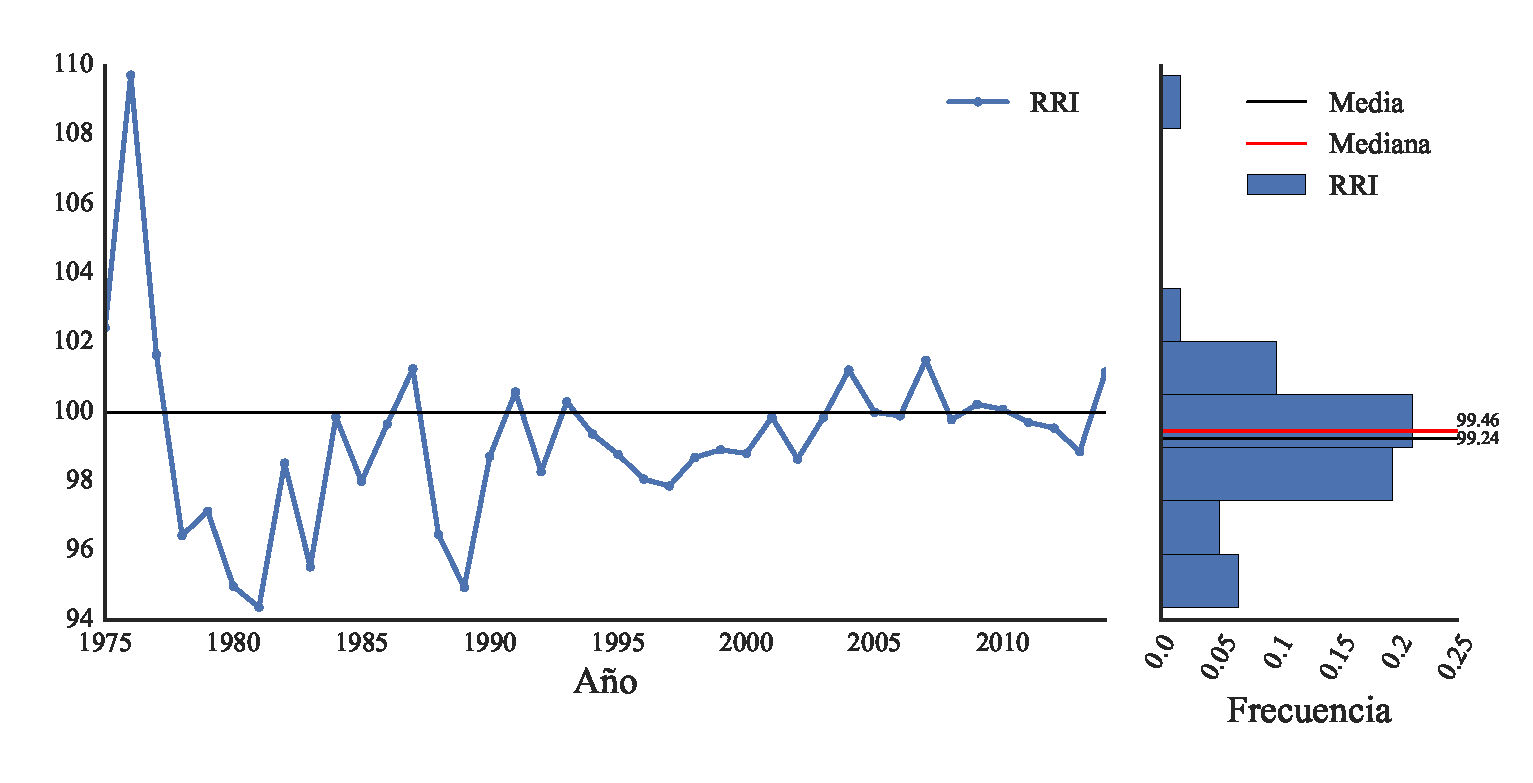
\includegraphics[width=300px]{rri_0.eps}
    \caption*{\textit{Fuente}: Elaboración propia con datos de \textit{World Bank API (WB)}}
    \label{rri}
\end{figure}

Cómo puede verse en al Figura \ref{rri}, la evolución de la relación real de intercambio de Chipre, gira en torno a un valor por debajo del 100\%, aproximadamente 99.46\% es el porcentaje medio y 99.24\% es el valor de la mediana, como puede constatarse en el histograma de la derecha, mas del 50\% de las observaciones la RRI de chipre se hallan con valores inferiores al 99.24\%, esto estrictamente indica que Chipre pierde bienestar con el comercio internacional, dado que el valor de lo que importa es superior a lo que exporta, lo que implica que para una mismca cantidad de exportaciones cada vez puede importar menos. En el periodo analizado sin duda Chipre ha perdido bienestar con el comercio internacional con más frecuencia que el que ha ganado.





\chapter{Evolución Del Comercio}
\label{cap2}

\begin{sidewaystable}[h]
    \centering
    \caption{Evolución de los Últimos 10 años del comercio de Chipre}
    \label{}
    \resizebox{\textwidth}{!}{%
    \begin{tabular}{lrrrrrrrrrrrr}
    \toprule
    {} &  \multicolumn{1}{|p{3cm}|}{\centering Importaciones de \\ BBSS (moneda local)} &  \multicolumn{1}{|p{3cm}|}{\centering Exportaciones de \\ BBSS (moneda local)} &  \multicolumn{1}{|p{3cm}|}{\centering Crecimiento nominal \\ de las importaciones (\%)} &  \multicolumn{1}{|p{3cm}|}{\centering Crecimiento nominal \\ de las exportaciones (\%)} &  \multicolumn{1}{|p{3cm}|}{\centering Crecimiento real \\ de las importaciones (\%)} &  \multicolumn{1}{|p{3cm}|}{\centering Crecimiento real \\ de las exportaciones (\%)} & \multicolumn{1}{|p{3cm}|}{\centering Saldo comercial \\ (LCU)} &  \multicolumn{1}{|p{3cm}|}{\centering Saldo Comercial \\ (\% PIB)} &  \multicolumn{1}{|p{3cm}|}{\centering Tasa de \\ Cobertura (\%)} &  \multicolumn{1}{|p{3cm}|}{\centering Tasa de\\ Apertura (\%)} & \multicolumn{1}{|p{3cm}|}{\centering  Penetración\\ de las Importaciones (\%)} &  \multicolumn{1}{|p{3cm}|}{\centering Propensión\\ Exportadora} \\
    Año &                                       &                                       &                                               &                                               &                                            &                                            &                        &                          &                        &                       &                                       &                         \\
    \midrule
    2000 & 7.155.010.000,00                     & 7.412.550.000,00                     & 14,38                                         & 13,81                                         & 9,21                                       & 8,79                                       & 257.540.000,00        & 2,44                     & 103,60                 & 138,27                & 69,62                                 & 70,36                  \\
    2001 & 7.265.740.000,00                     & 7.787.330.000,00                     & 1,55                                          & 5,06                                          & -0,19                                      & 2,18                                       & 521.590.000,00        & 4,60                     & 107,18                 & 132,73                & 67,15                                 & 68,66                  \\
    2002 & 7.273.030.000,00                     & 7.411.900.000,00                     & 0,10                                          & -4,82                                         & -0,36                                      & -4,09                                      & 138.870.000,00        & 1,18                     & 101,91                 & 124,45                & 62,37                                 & 62,81                  \\
    2003 & 7.224.510.000,00                     & 7.419.710.000,00                     & -0,67                                         & 0,11                                          & -0,97                                      & -1,40                                      & 195.200.000,00        & 1,53                     & 102,70                 & 114,81                & 57,52                                 & 58,17                  \\
    2004 & 7.900.090.000,00                     & 7.882.900.000,00                     & 9,35                                          & 6,24                                          & 6,95                                       & 2,49                                       & -17.190.000,00        & -0,13                    & 99,78                  & 114,94                & 57,46                                 & 57,41                  \\

    2005 &                      8.333.840.000,00 &                      8.254.850.000,00 &                                          5,49 &                                          4,72 &                                       1,57 &                                       2,05 &         -78.990.000,00 &                    -0,54 &                  99,05 &                112,92 &                                 56,42 &                   56,19 \\
    2006 &                      9.019.310.000,00 &                      8.549.730.000,00 &                                          8,23 &                                          3,57 &                                       5,70 &                                       1,27 &        -469.580.000,00 &                    -2,97 &                  94,79 &                110,94 &                                 55,31 &                   53,99 \\
    2007 &                     10.159.530.000,00 &                      9.326.470.000,00 &                                         12,64 &                                          9,08 &                                      10,46 &                                       5,28 &        -833.060.000,00 &                    -4,81 &                  91,80 &                112,45 &                                 55,94 &                   53,82 \\
    2008 &                     11.440.420.000,00 &                      9.417.380.000,00 &                                         12,61 &                                          0,97 &                                       7,74 &                                      -1,72 &      -2.023.040.000,00 &                   -10,78 &                  82,32 &                111,13 &                                 55,02 &                   50,18 \\
    2009 &                      9.550.060.000,00 &                      8.721.350.000,00 &                                        -16,52 &                                         -7,39 &                                     -16,05 &                                      -7,28 &        -828.710.000,00 &                    -4,50 &                  91,32 &                 99,18 &                                 49,61 &                   47,34 \\
    2010 &                     10.157.580.000,00 &                      9.095.460.000,00 &                                          6,36 &                                          4,29 &                                       4,52 &                                       2,63 &      -1.062.120.000,00 &                    -5,57 &                  89,54 &                101,00 &                                 50,47 &                   47,71 \\
    2011 &                     10.319.010.000,00 &                      9.653.110.000,00 &                                          1,59 &                                          6,13 &                                      -0,62 &                                       4,21 &        -665.900.000,00 &                    -3,42 &                  93,55 &                102,49 &                                 51,20 &                   49,54 \\
    2012 &                     10.028.060.000,00 &                      9.653.370.000,00 &                                         -2,82 &                                          0,00 &                                      -4,60 &                                      -1,66 &        -374.690.000,00 &                    -1,93 &                  96,26 &                101,39 &                                 50,68 &                   49,73 \\
    2013 &                      8.759.650.000,00 &                      9.209.850.000,00 &                                        -12,65 &                                         -4,59 &                                     -13,61 &                                      -4,99 &         450.200.000,00 &                     2,48 &                 105,14 &                 99,18 &                                 49,58 &                   50,83 \\
    2014 &                      9.220.300.000,00 &                      9.704.100.000,00 &                                          5,26 &                                          5,37 &                                       8,07 &                                       5,72 &         483.800.000,00 &                     2,76 &                 105,25 &                108,10 &                                 54,17 &                   55,43 \\

    \bottomrule
\end{tabular}}
\caption*{\textit{Fuente}: Elaboración propia con datos de World Bank API.}
\end{sidewaystable}

\section{Nominal}


\begin{figure}[htb]
    \caption{Evolución de las exportaciones (por uno) y su frecuencia.}
    \centering
    \includegraphics[width=300px]{ev_nominal.pdf}
    \caption*{\textit{Fuente}: Elaboración propia con datos de World Bank API.}
    \label{ev_nominal}
\end{figure}

Tanto las importaciones cómo las exportaciones se han visto afectadas nominalmente en 2008 por la crisis económica, se puede ver en la caída de éstas en el gráfico. En los últimos 10 años, el crecimiento de ambas variables ha estado girando en torno al 2\% siendo las exportaciones ligeramente superior a las importaciones haciendo que el crecimiento del saldo exterior sea positivo pero muy discreto de magnitud de un 0.2\%. Es interesante que ver que sólo el 20\% de los años el crecimiento de las exportaciones presentó valores negativos (30\% para las importaciones) esto se debe principalmente, cómo veremos en el siguiente gráfico, a la inflación.


\section{Real}


\begin{table}[]
\centering
\caption{Evolución de las importaciones de Chipre.}
\label{tab2}
\begin{tabular}{@{}lrr@{}}
\toprule
date & \multicolumn{1}{l}{\begin{tabular}[c]{@{}l@{}}Importaciones de \\ bienes y servicios \\ (constante LCU)\end{tabular}} & \multicolumn{1}{l}{\begin{tabular}[c]{@{}l@{}}Importaciones de \\ bienes y servicios \\ (corriente LCU)\end{tabular}} \\ \midrule
1980 & 2.676.118.100,00                                                                                                      & 819.274.400,00                                                                                                        \\
1981 & 2.743.072.900,00                                                                                                      & 947.761.300,00                                                                                                        \\
1982 & 3.094.066.300,00                                                                                                      & 1.124.943.200,00                                                                                                      \\
1983 & 3.264.572.800,00                                                                                                      & 1.242.495.000,00                                                                                                      \\
1984 & 3.798.964.600,00                                                                                                      & 1.533.298.900,00                                                                                                      \\
1985 & 3.626.378.900,00                                                                                                      & 1.489.900.500,00                                                                                                      \\
1986 & 3.229.223.700,00                                                                                                      & 1.324.507.800,00                                                                                                      \\
1987 & 3.688.343.200,00                                                                                                      & 1.529.027.400,00                                                                                                      \\
1988 & 4.176.573.800,00                                                                                                      & 1.824.615.500,00                                                                                                      \\
1989 & 5.015.381.800,00                                                                                                      & 2.308.833.100,00                                                                                                      \\
1990 & 5.302.331.700,00                                                                                                      & 2.493.703.900,00                                                                                                      \\
1991 & 5.407.130.200,00                                                                                                      & 2.609.205.300,00                                                                                                      \\
1992 & 6.403.969.100,00                                                                                                      & 3.214.904.500,00                                                                                                      \\
1993 & 5.226.227.600,00                                                                                                      & 2.681.479.100,00                                                                                                      \\
1994 & 5.597.598.500,00                                                                                                      & 2.999.449.800,00                                                                                                      \\
1995 & 6.531.110.000,00                                                                                                      & 5.192.630.000,00                                                                                                      \\
1996 & 6.842.650.000,00                                                                                                      & 5.636.820.000,00                                                                                                      \\
1997 & 6.926.900.000,00                                                                                                      & 5.909.750.000,00                                                                                                      \\
1998 & 6.963.940.000,00                                                                                                      & 5.998.680.000,00                                                                                                      \\
1999 & 7.133.060.000,00                                                                                                      & 6.255.730.000,00                                                                                                      \\
2000 & 7.790.250.000,00                                                                                                      & 7.155.010.000,00                                                                                                      \\
2001 & 7.775.370.000,00                                                                                                      & 7.265.740.000,00                                                                                                      \\
2002 & 7.747.590.000,00                                                                                                      & 7.273.030.000,00                                                                                                      \\
2003 & 7.672.140.000,00                                                                                                      & 7.224.510.000,00                                                                                                      \\
2004 & 8.205.030.000,00                                                                                                      & 7.900.090.000,00                                                                                                      \\
2005 & 8.333.830.000,00                                                                                                      & 8.333.840.000,00                                                                                                      \\
2006 & 8.809.070.000,00                                                                                                      & 9.019.310.000,00                                                                                                      \\
2007 & 9.730.760.000,00                                                                                                      & 10.159.530.000,00                                                                                                     \\ \bottomrule
\end{tabular}
\end{table}


\begin{figure}[htb]
    \caption{Evolución de las importaciones (por uno) y su frecuencia.}
    \centering
    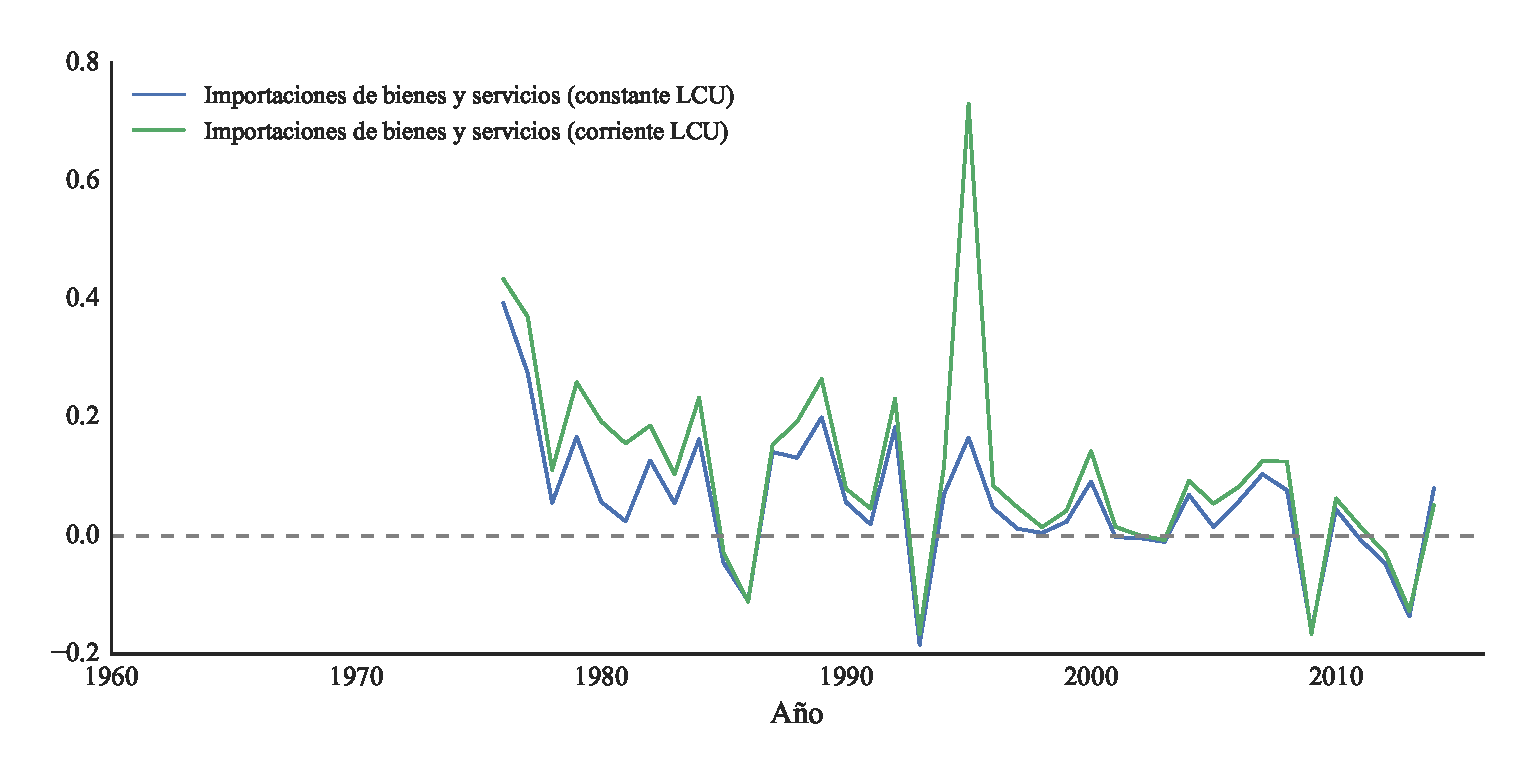
\includegraphics[width=300px]{ev_m.eps}
    \label{ev_m}
\end{figure}


\chapter{Distribución Geográfica De M Y X}
\label{cap3}

\begin{figure}[!ht]
    \centering
    \caption{}
    \includegraphics[width=300px]{pie_mgeo.pdf}
    \caption*{\textit{Fuente}: Elaboración propia con datos de \textit{PC-TAS}}
    \label{}
\end{figure}

\begin{figure}[!ht]
    \centering
    \caption{}
    \includegraphics[width=300px]{bar_mgeo.pdf}
    \caption*{\textit{Fuente}: Elaboración propia con datos de \textit{PC-TAS}}
    \label{}
\end{figure}

Los principales orígenes de las importaciones de Chipre son países de la propia unión europea como muestra la Figura REF, pero destaca sobre el resto las importaciones procedentes de Grecia con casi el doble de peso sobre el esto, diferencia que se ha mantenido desde 2007 hasta 2011.
Estas relaciones se pueden explicar con el pasado geopolítico de Chipre, que pasó a estar a menos de UK, luego Grecia y con una cultura... continuar

\begin{figure}[!ht]
    \centering
    \caption{}
    \includegraphics[width=300px]{pie_xgeo.pdf}
    \caption*{\textit{Fuente}: Elaboración propia con datos de \textit{PC-TAS}}
    \label{}
\end{figure}

\begin{figure}[!ht]
    \centering
    \caption{}
    \includegraphics[width=300px]{bar_xgeo.pdf}
    \caption*{\textit{Fuente}: Elaboración propia con datos de \textit{PC-TAS}}
    \label{}
\end{figure}


Las exportaciones de Chipre tienen como principales destinos, Grecia, Para Buques, Reino Unido, Alemania y Rumanía, que juntas tiene un peso de 58.69\% en 2007 y 56.79\% en 2011. Cómo puede verse en la Figura REF, las exportaciones de 2007 hacia Grecia y Para Buques aumentaron en 2011, mientras que el resto disminuyeron.
Los destinos concuerdan con la historia Chipriota, fué una colonia y de Reino Unido, y formó parte de Grecia, esta dependencia del pasado ha hecho que se mantenga hasta hoy en día nexos comerciales fuertes.

FALTA MODELO DE GRAVEDAD


\chapter{Competitividad Precio O Coste}
\label{cap4}

\chapter{Competitividad Estructural}
\label{cap5}

\chapter{Especialización comercial}

ESPECIALIZACIÓN COMERCIAL

INDICE DE DEPENDENCIA

Para todo país $h$ y el sector $i$

\begin{equation}
IDep^h_i = \frac{\frac{M^h_i}{\sum_i M^h_i}}{\frac{\sum_h M^h_i}{\sum_h \sum_i M^h_i}} 100
\end{equation}

INDICE DE ESPECIALIZACIÓN

\begin{equation}
IEsp^h_i = \frac{\frac{X^h_i}{\sum_i X^h_i}}{\frac{\sum_h X^h_i}{\sum_h \sum_i X^h_i}} 100
\end{equation}

SALDO COMERCIAL RELATIVO

\begin{equation}
SCR_i = \frac{X_i - M_i}{X_i + M_i} 100
\end{equation}

IMPORTANCIA RELATIVA DEL SECTOR EN LAS IMPORTACIONES Y EXPORTACIONES.

\begin{equation}
IRX_i = \frac{X_i}{\sum_i X_i}
\end{equation}

\begin{equation}
IRM_i = \frac{M_i}{\sum_i M_i}
\end{equation}

\begin{figure}[!ht]
    \centering
    \caption{}
    \includegraphics[width=300px]{cuadrantes2.pdf}
    \caption*{\textit{Fuente}: Elaboración propia con datos de \textit{PC-TAS}}
    \label{}
\end{figure}


\begin{figure}[!ht]
    \centering
    \caption{}
    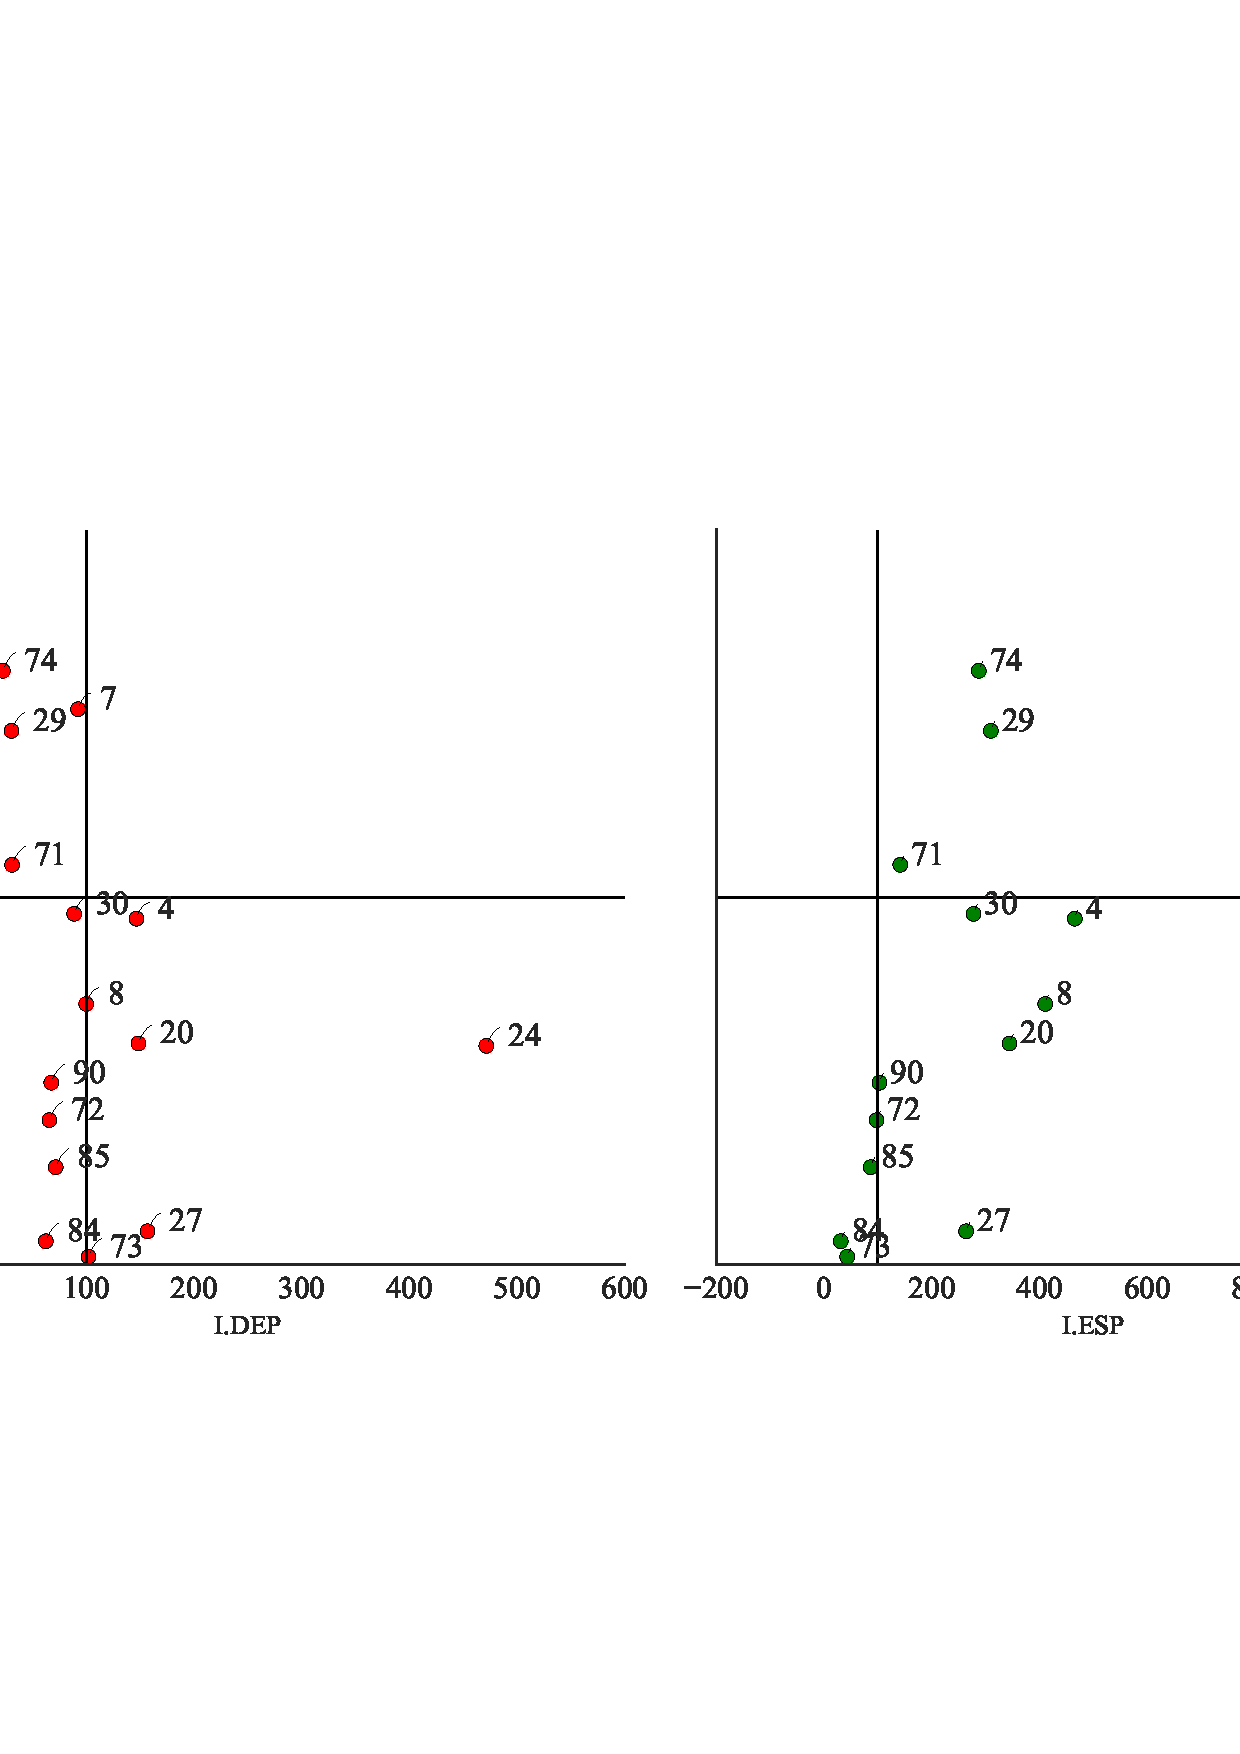
\includegraphics[width=400px]{cuadrantes.pdf}
    \caption*{\textit{Fuente}: Elaboración propia con datos de \textit{PC-TAS}}
    \label{}
\end{figure}


\chapter{Comercio Intraindustrial}

\chapter{Política Comercial}

\chapter{Resumen y Conclusiones}

\chapter{Anexo}

En el Capítulo \ref{cap1} se han usado los siguientes indicadores:

\begin{enumerate}

    \item BALANZA COMERCIAL

    $$X - M$$
    \item TASA DE COBERTURA

    $$\frac{X}{M}100$$
    \item PENETRACIÓN DE LAS IMPORTACIONES

    $$\frac{M}{\text{PIB} + M - X} 100$$
    \item GRADO DE APERTURA

    $$\frac{X+M}{\text{PIB}} 100$$
    \item PROPENSIÓN EXPORTADORA

    $$\frac{X}{\text{PIB}} 100$$

\end{enumerate}

Para el Capítulo \ref{cap3}:

\begin{enumerate}
    \item COMPETITIVIDAD PRECIO O COSTE
    \begin{enumerate}
        \item Indices de tipo de cambio efectivo real
        \item Tipo de cambio oficial
        \item Tasa de inflación
    \end{enumerate}

\item ESPECIALIZACIÓN COMERCIAL

\item  INDICE DE DEPENDENCIA

Para todo país $h$ y el sector $i$

$$IDep^h_i = \frac{\frac{M^h_i}{\sum_i M^h_i}}{\frac{\sum_h M^h_i}{\sum_h \sum_i M^h_i}} 100$$

\item  INDICE DE ESPECIALIZACIÓN

$$IEsp^h_i = \frac{\frac{X^h_i}{\sum_i X^h_i}}{\frac{\sum_h X^h_i}{\sum_h \sum_i X^h_i}} 100$$

\item  SALDO COMERCIAL RELATIVO

$$SCR_i = \frac{X_i - M_i}{X_i + M_i} 100$$

\item IMPORTANCIA RELATIVA DEL SECTOR EN LAS IMPORTACIONES Y EXPORTACIONES.

$$IRX_i = \frac{X_i}{\sum_i X_i}$$

$$IRM_i = \frac{M_i}{\sum_i M_i}$$

\item COMERCIO INTRAINDUSTRIAL

$$IGL_i = \frac{X_i + M_i - |X_i - M_i|}{X_i + M_i}100$$

$$IGL_{agg} = \frac{\sum_i(X_i + M_i) - \sum_i |X_i - M_i|}{\sum_i (X_i + M_i)}100$$

\end{enumerate}


\cleardoublepage
\addcontentsline{toc}{chapter}{Bibliografía}
\bibliographystyle{apalike}
\bibliography{biblio.bib} % yyyy.bib es el fichero donde está salvada la bibliografía.


\end{document}
